% Preamble
% ========
\documentclass[10pt,letterpaper]{article}

% Define packages to use
\usepackage{natbib}
\usepackage[dvips]{graphicx,color}
\usepackage{amsmath,amssymb}
\usepackage{caption}
\usepackage[dvipdfm,colorlinks,linkcolor=blue,citecolor=blue,urlcolor=blue]{hyperref}

% Redefine default page
\setlength{\textheight}{9in}  % 1" above and below
\setlength{\textwidth}{6.75in}   % 0.5" left and right
\setlength{\oddsidemargin}{-0.25in}

% Redefine default paragraph
\setlength{\parindent}{0pt}
\setlength{\parskip}{1ex plus 0.5ex minus 0.2ex}

% Define caption width and default fonts
\setlength{\captionmargin}{0.5in}
\renewcommand{\captionfont}{\sffamily}
\renewcommand{\captionlabelfont}{\bfseries\sffamily}

% Define commands for super- and subscript in text mode
\newcommand{\superscript}[1]{\ensuremath{^\textrm{#1}}}
\newcommand{\subscript}[1]{\ensuremath{_\textrm{#1}}}


% Document
% ========
\begin{document}
\thispagestyle{empty}

% Heading
\begin{center}
  {\Large\bfseries Implementation of a new infrared sea surface emissivity model in the Community Radiative Transfer Model (CRTM)}\vspace{1.0em}
  
  {\bfseries Paul F. van Delst\superscript{a}, Nicholas R. Nalli\superscript{b}, and John C. Derber\superscript{c}}\vspace{1.0em}
  
  a. SAIC, NOAA/NWS/NCEP/EMC, Joint Center for Satellite Data Assimilation\\
  b. PSGS Inc., NOAA/NESDIS/STAR\\
  c. NOAA/NWS/NCEP/EMC, Joint Center for Satellite Data Assimilation\vspace{1.0em}
  
  Submitted for the 2\superscript{nd} Workshop on Remote Sensing and Modeling of Surface Properties.
\end{center}

% Main text
The CRTM is used in the NCEP/EMC\footnote{National Centers for Environmental Prediction/Enivironmental Modeling Center} data assimilation systems to simulate satellite radiance observations. The current infrared (IR) sea surface emissivity model component of the CRTM has been in use since 2006 and is based on \cite{WuSmith_1997} in which the reflected sea surface emission is taken into account.

Recent work \citep{HanafinMinnett_2005,Nalli_2008a,Nalli_2008b} has shown that this methodology will underestimate the effective emissivity at larger zenith angles due to the quasi-specular reflection of downwelling atmospheric radiance into the sensor field-of-view. A comparison of computed emissivities for a large view angle is shown in figure \ref{fig:wu_nalli_comparison}. The difference between the Wu-Smith and Nalli model emissivities in the longwave IR window region (800-950cm\superscript{-1}) is around 0.01, or 1\%. For blackbody emission at typical sea surface temperatures, this is roughly equivalent to a brightness temperature error of 0.7K. When the reflected downwelling atmospheric radiation is included, this error reduces to a still significant 0.5K \citep{WuSmith_1996}.

The impact of the new IR sea surface emissivity model in the data assimilation system at NCEP/EMC will be evaluated. In addition, because the CRTM IR sea surface emissivity models are implemented via look-up-tables as functions of frequency, wind speed and view angle, interpolation artifacts in the adjoint model will be described.

\begin{figure}[htb]
  \centering
  \includegraphics[bb=70 305 540 495,clip,scale=0.9]{graphics/wu_nalli_comparison.eps}
  \caption{Comparison of Wu-Smith emissivities with that of Nalli using \citet{CoxMunk_1954} (CM) and \citet{EbuchiKizu_2002} (EK) wave slope statistics for a wind speed of 6ms\superscript{-1} and zenith angle of 60$^\circ$.}
  \label{fig:wu_nalli_comparison}
\end{figure}

\bibliographystyle{plainnat}
\bibliography{bibliography}
\end{document}

